%Plan

\subsection{GENIE and the comparisons}
GENIE applies theoretical physics models, composed of both physical and unphysical parameters, to detector geometries and materials to build experiment-specific neutrino interaction predictions \cite{genie}. The collaboration is in the process of improving configurations of these models for the purpose of optimising the accuracy of the predictions.

    An archive of experimental data is publicly available, and provides the key ingredient to this configuration update. Comparing the models with these data sets allows for a direct performance evaluation of the predictions, whilst fitting the models to the data enables the parameters to be tuned and consequently improve the prediction.

Summaries of the configuration of the GENIE models are as follows:

\begin{figure}[h!]
    \centering
    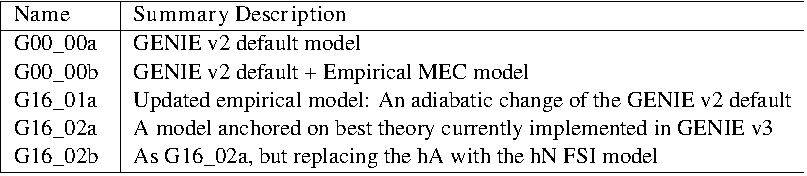
\includegraphics[width=\textwidth]{images/model_summaries.pdf}
    \caption{A brief overview the features which make up the individual model configurations in GENIE. These models will eventually all be tuned.}
    \label{fig:modelConfigs}
\end{figure}


The model used in the tuning addresses the observation of the abnormalities seen in recent experiments by incorporating the MEC interaction, Figure~\ref{fig:MECSchem} \cite{MEC} describes this interaction schematically in terms of the models involved. 

\begin{figure}[h!]
    \centering
    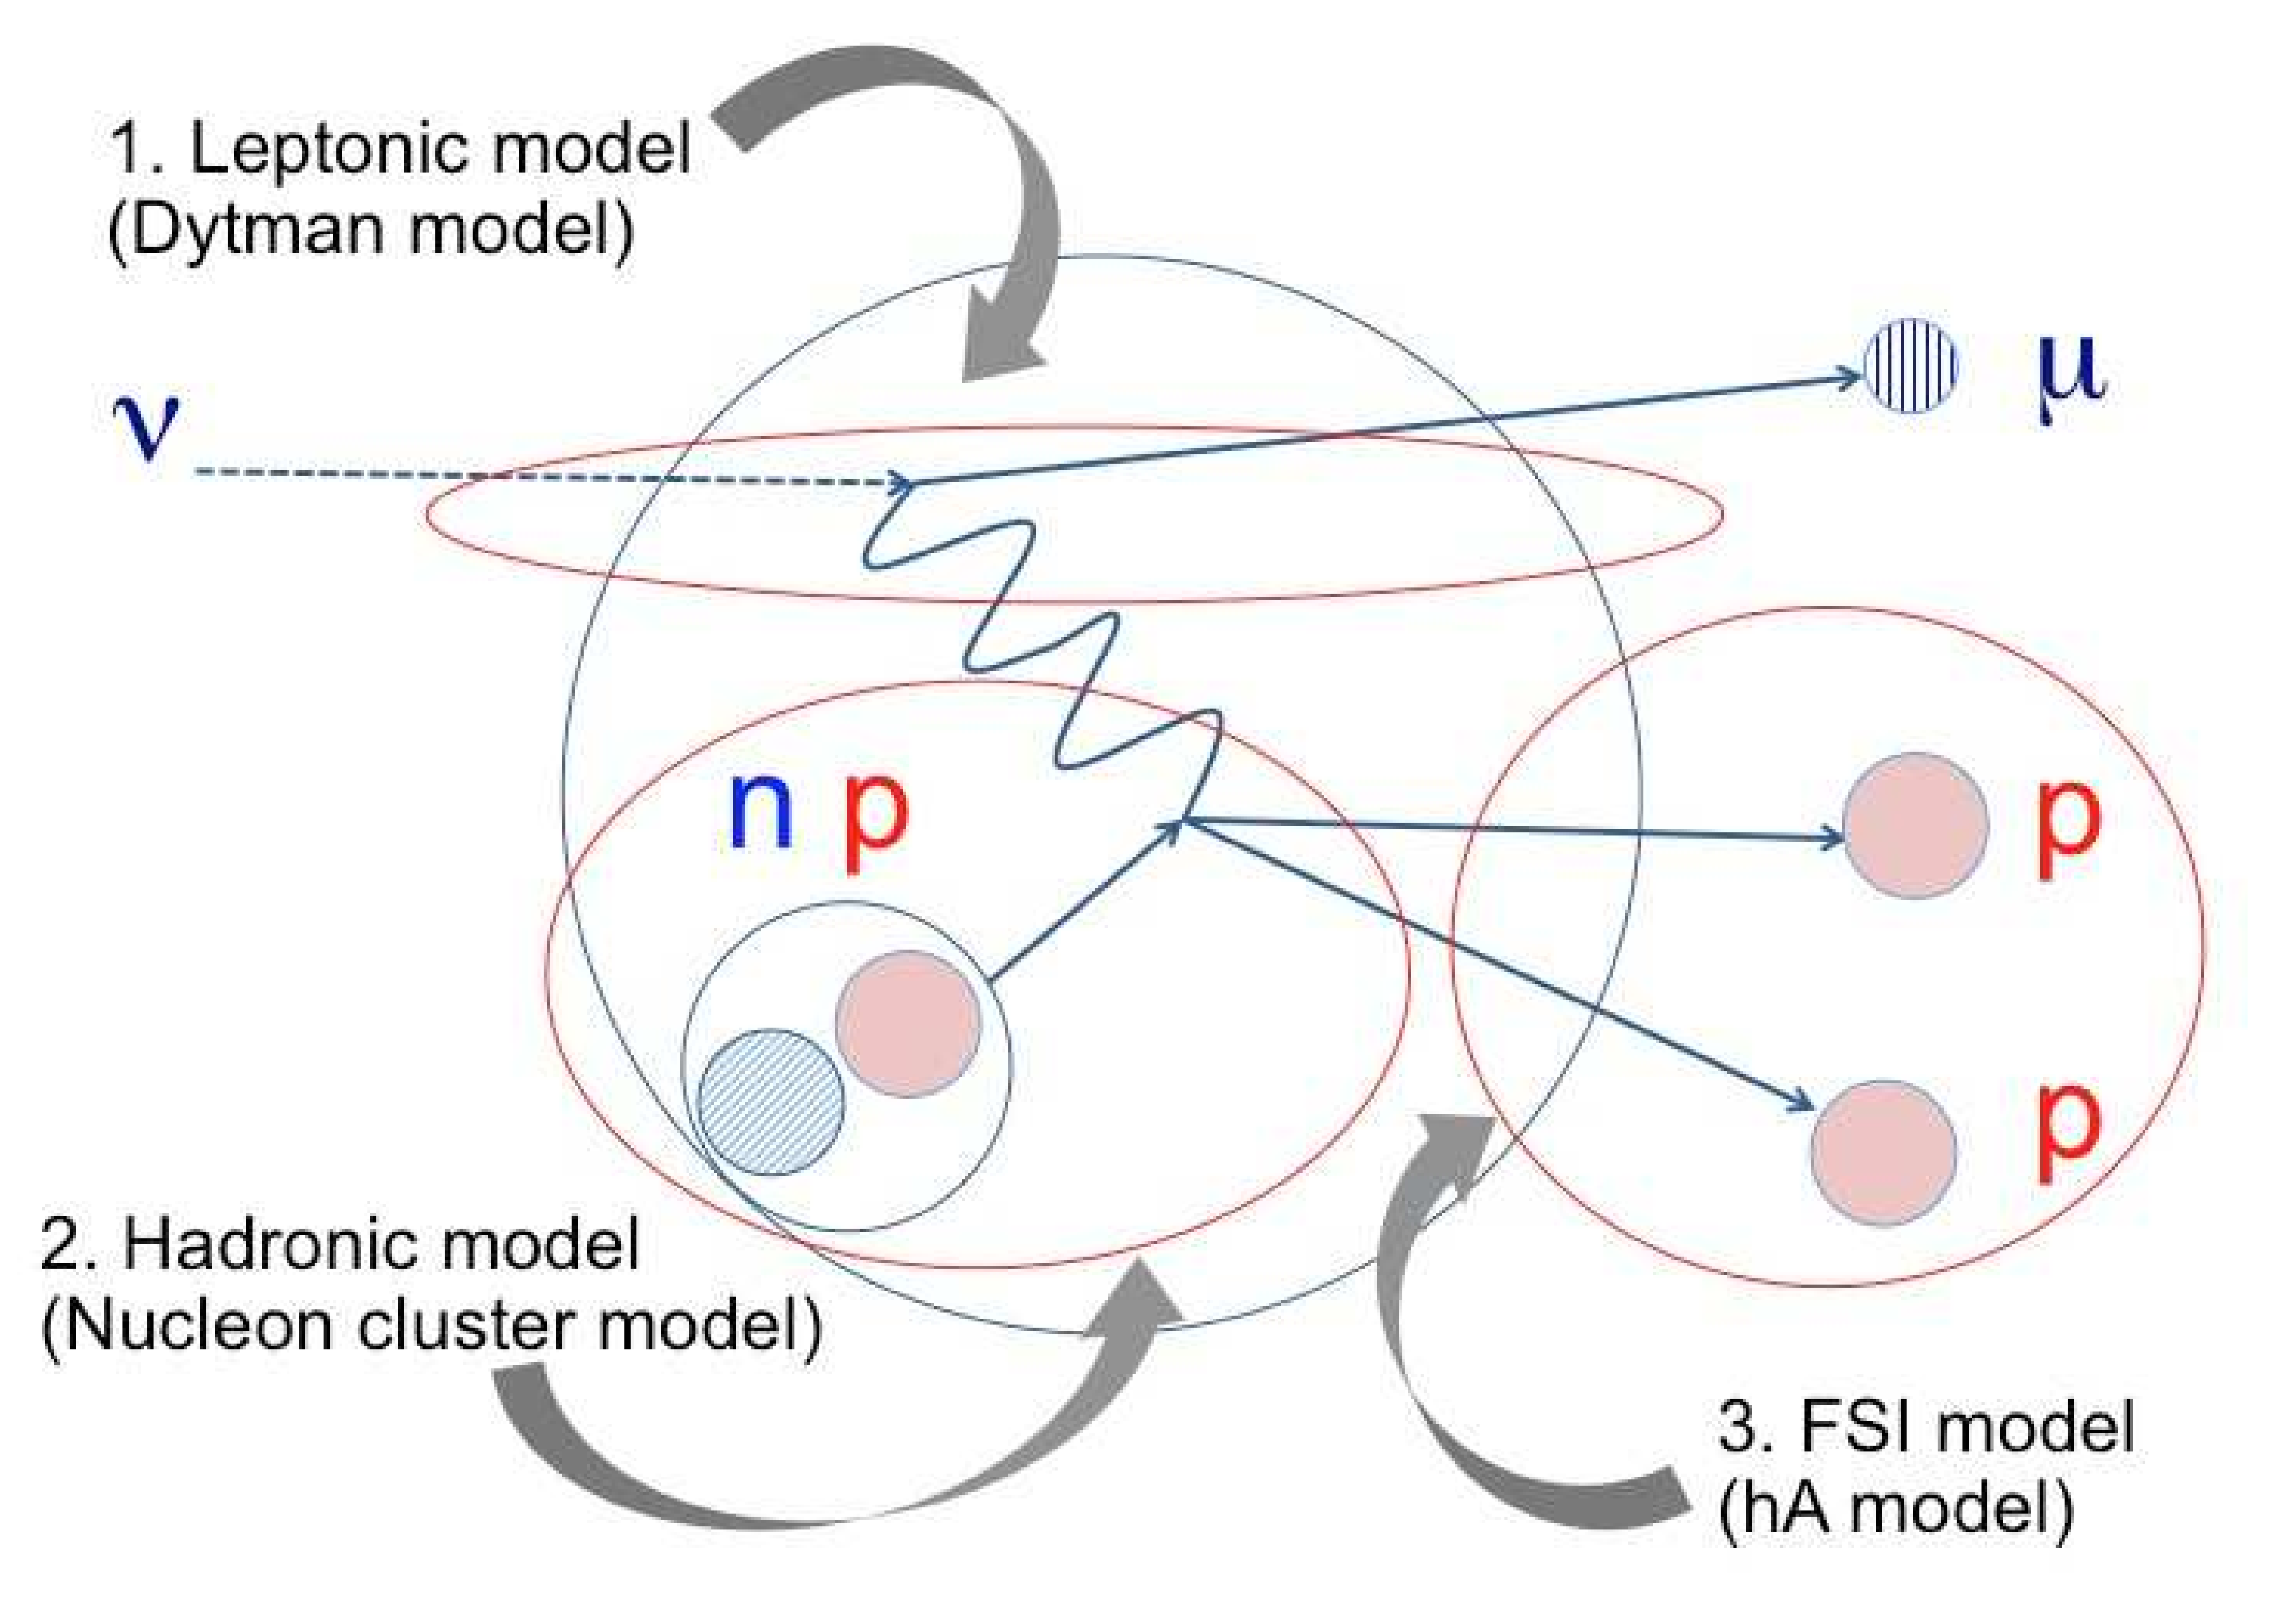
\includegraphics[width=.6\textwidth]{images/mec_model_genie.png}
    \caption{The models involved in the construction of the MEC model in neutrino event generation.}
    \label{fig:MECSchem}
\end{figure}

\begin{itemize}
    \item Publicly available datasets
    \item Comparisons
    \begin{itemize}
        \item MiniBooNE
        \item T2K
        \item Minerva
    \end{itemize}
    \item Tensions
\end{itemize}

\subsection{Process}
\begin{itemize}
    \item Motivate global fit
    \item Description of global fit
    \item Professor
    \begin{itemize}
        \item How it works
        \item Schematic
    \end{itemize}
\end{itemize}

\subsection{Results}
\begin{itemize}
    \item Results 
\end{itemize}



\clearpage
